%!TEX root = ../TTK4900-MHT.tex

\chapter{MHT Module}\label{chapter:mht-module}
To create a complete tracking \emph{system}, rather than a tracking \emph{algorithm}, it is often necessary  to complement the main algorithm with other support modules. The system or a module if it is a part of a bigger system presented here is an extension of~\cite{Liland_2017}.
The aim of this chapter is to provide a complete walkthrough of the the track oriented MHT system presented in this thesis. The motion model which is used throughout the entire tracking system when predicting and filtering target behaviour is explained first. Next follows an overview of the algorithm used to initiate new tracks into the MHT algorithm. Followed by the entire MHT tracking algorithm, with all its sub-routines and bookkeeping. 

\section{Motion Model}\label{sec:motion-model}
A local Cartesian NED-frame will be used throughout this thesis, with the assumption than all input sensors are transformed to this local frame. In real life, when working on an approximated local Cartesian frame is doable as long as the area in question is reasonable small. A global geodetic frame would be preferable, but will yield non-linear motion equations. The state of the targets are modelled with four states
\begin{equation}
\V{x} = \begin{bmatrix}
x & y & \dot{x} & \dot{y}
\end{bmatrix}^T
\label{eq:state_vector}
\end{equation}
where the \(x\)-axis is pointing east and the \(y\)-axis is pointing north. The two latest states are the velocity in their respective direction. 

Since modelling the behaviour of any ship under unknown command is next to impossible, a common assumption in tracking theory is to assume that everyone will continue on as usual. Although simple, this model captures the essence of most vessels at sea, and when looking at maritime training, regulation and best-practice, they all dictates that vessels should hold steady course and change course in clear decisive turns. To give room in our model for manoeuvring a white noise is added on the states covariance. 
\begin{equation}
\V{x}(k+1) = \M{\Phi} \V{x}(k) + \M{\Gamma} \V{w}(k) \qquad \V{w} \sim \mathcal{N}(0;\M{Q})
\label{eq:motion_model}
\end{equation}
Where 
\begin{equation}
\begin{split}
\M{\Phi} 	&= \text{the state transition matrix} \\
\M{\Gamma}	&= \text{the disturbance matrix} \\
\V{w}		&= \text{the process noise}
\end{split}
\end{equation}
and 
\begin{equation*}
\M{\Phi} =	\begin{bmatrix}
1 & 0 & T & 0 \\
0 & 1 & 0 & T \\
0 & 0 & 1 & 0 \\
0 & 0 & 0 & 1 \\
\end{bmatrix}
\quad
\M{Q}	= \sigma_v^2 \begin{bmatrix}
\frac{T^3}{3} 	& 0 				& \frac{T^2}{2}	& 0 			\\
0 				& \frac{T^3}{3}  	& 0 			& \frac{T^2}{2}	\\
\frac{T^2}{2}	& 0					& T				& 0				\\
0				& \frac{T^2}{2}		& 0				& T				\\
\end{bmatrix}
\end{equation*}



\section{Track Initiation}
New tracks are initiated with 2/2 \& m/n logic~\cite{Vo2015} on the crumbles after each MHT iteration.

\section{MHT Overview}
\begin{figure}[H]
\centering
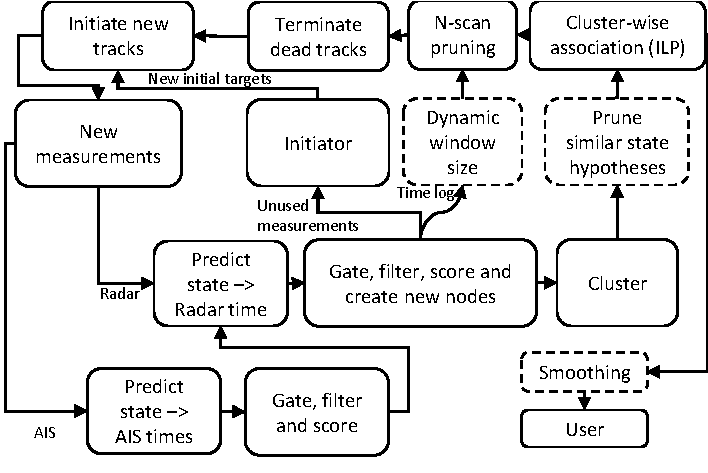
\includegraphics[width = .8\textwidth]{algorithm_flowchart.pdf}
\caption{Algorithm flowchart}
\label{fig:algorithm_flow}
\end{figure}

\section{Predict target position}
\begin{equation}
\begin{split}
\V{\bar{x}}(k+1) 	&= \M{\Phi} \V{\hat{x}}(k) \\
\M{\bar{P}}(k+1)	&= \M{\Phi} \M{\hat{P}}(k)  \M{\Phi}^T + \M{Q} \\
\end{split}
\label{eq:kalman_timeUpdate}
\end{equation}

\section{Gate and Create new hypotheses}
\begin{equation}
\begin{gathered}
\M{S}	= \M{H} \M{\bar{P}} \M{H}^T + \M{R} \\
\V{\tilde{z}} = \V{z} - \M{H}\V{\bar{x}} \\
\V{\tilde{z}}^T	\M{S}^{-1} \V{\tilde{z}} \leq \eta^2
\label{eq:gate}
\end{gathered}
\end{equation}

\subsection{Zero hypothesis}
To account for the possibility that the target is not present in this scan, a \emph{zero} hypothesis, or \emph{dummy} hypothesis as it is sometimes called, is generated with the predicted state and covariance.

\subsection{Pure radar hypotheses}
For every radar measurement inside the gate in (\ref{eq:gate}), a new track hypothesis is generated with filtered state and covariance according to regular Kalman measurement update equations (\ref{eq:kalman_measurementUpdate}).
\begin{equation}
\begin{split}
\V{\tilde{y}}	&= \V{z} - \M{H} \V{\bar{x}} \\
\M{S}			&= \M{H} \M{\bar{P}} \M{H}^T + \M{R} \\
\M{K} 			&= \M{\bar{P}} \M{H}^T \M{S}^{-1} \\
\V{\hat{x}}(k) 	&= \V{\bar{x}} + \M{K} \V{\tilde{y}} \\
\M{\hat{P}}(k) 	&= \left( \M{I} - \M{K} \M{H} \right) \M{\bar{P}}
\end{split}
\label{eq:kalman_measurementUpdate}
\end{equation}

\subsection{Combined radar and AIS hypotheses}\label{subsec:combined_radar_and_ais_hypotheses}
As elaborated in Section \ref{sec:ais_preprocessing} all AIS measurements are preprocessed to remove out-of-order messages and ID-swap errors. And for each radar scan only the latest AIS update from each target (\gls{mmsi} number) are passed through to the MHT tracking loop.

For every (predicted) \gls{ais} measurement, there are generated a new complete set of hypotheses consisting of the \gls{ais} measurement and all the radar measurements inside the gate. This will lead to a large number of new hypotheses, but since the number of \gls{ais} measurements inside any gate at any time will seldom be larger than one, and in most cases zero, this will not cause any substantially larger explosion in the number of track hypotheses that the already exponentially nature of any \gls{mht}.% Since both the radar- and \gls{ais} measurement have the same process noise, the fused estimate will have an uncertainty area about 70 percent of the pure radar measurement, whereas the uncertainty would be 50 percent without common process noise~\cite{Bar-Shalom1986}.

Since the AIS measurements originates before the radar measurement, the fusion is carried out in two steps as a sequential update~\cite{Bar-Shalom1995}. 
\begin{figure}[H]
\centering
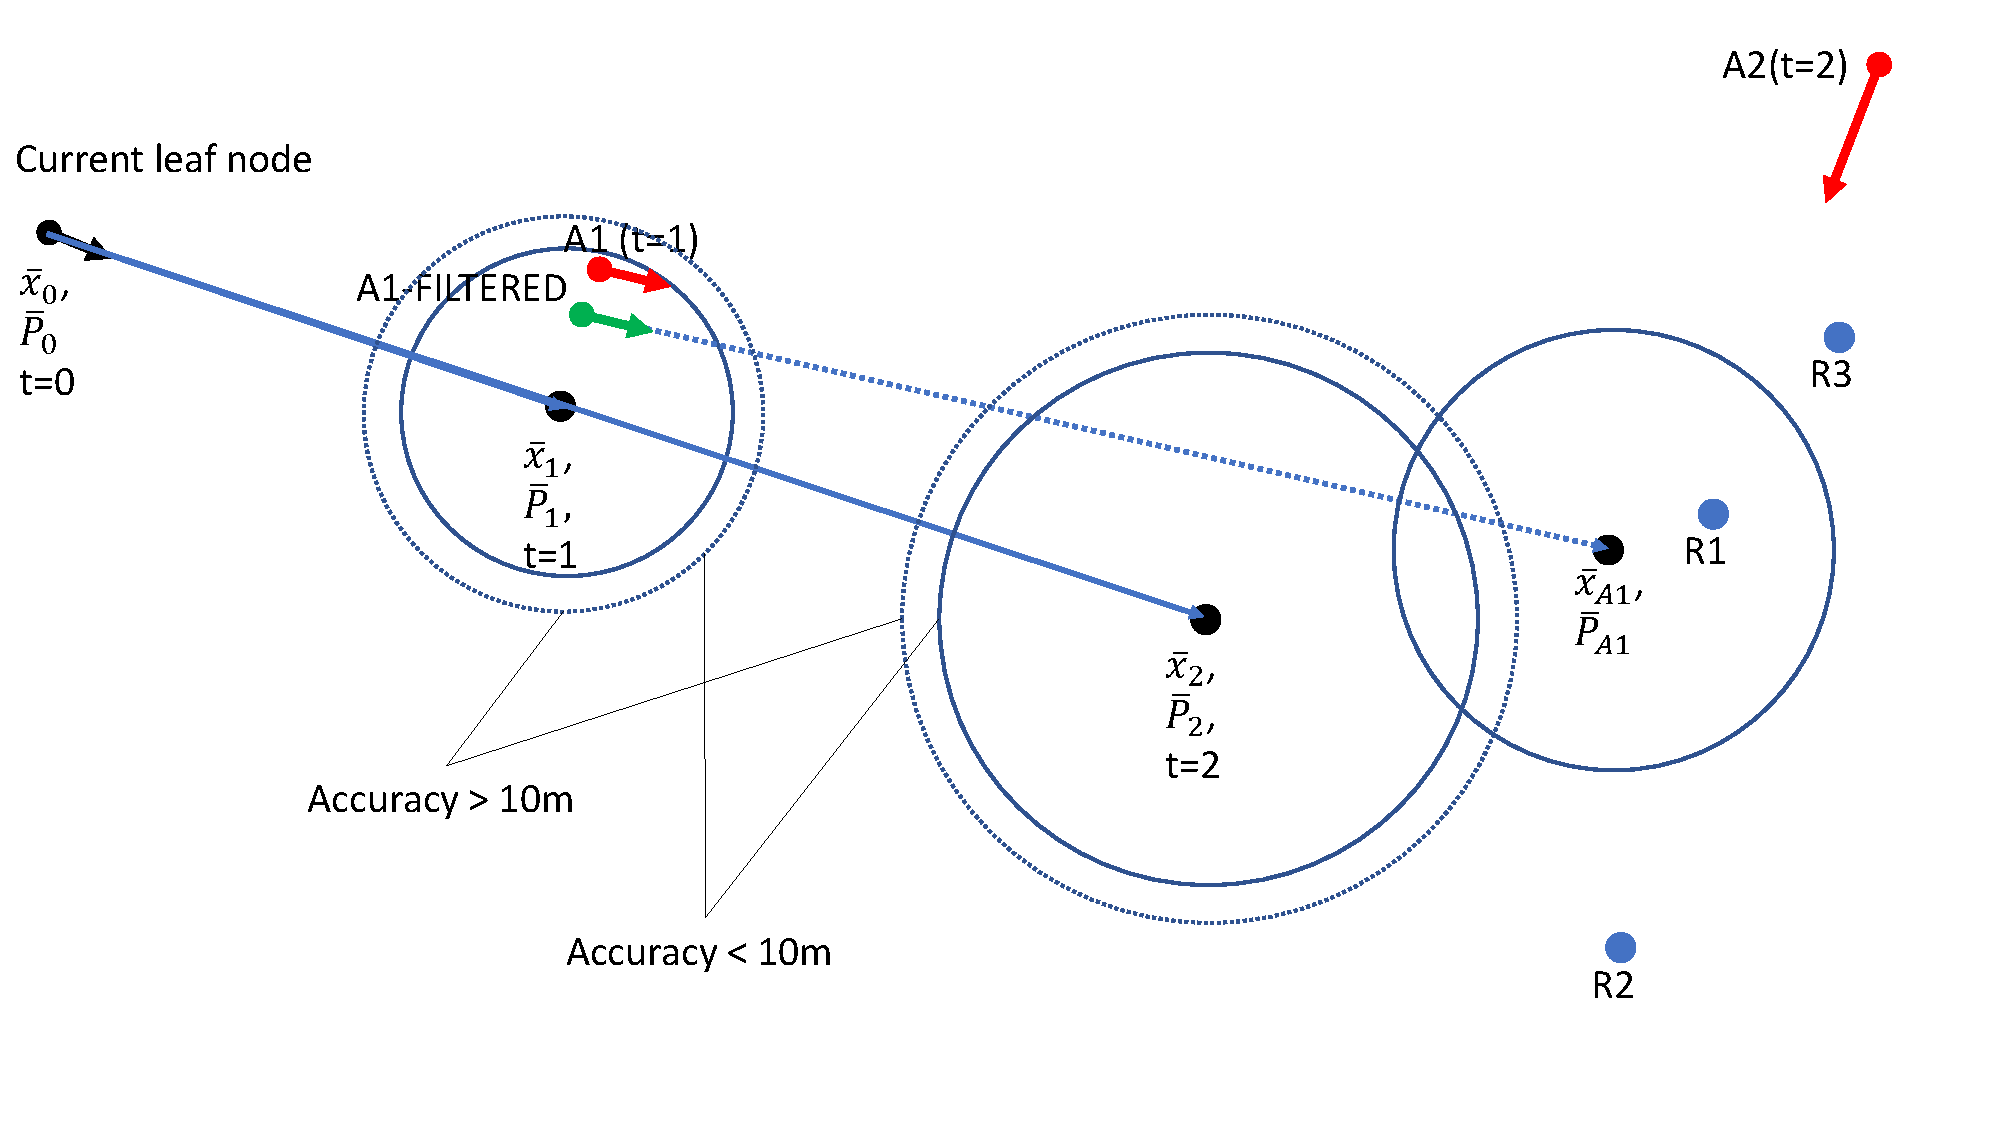
\includegraphics[width = .8\textwidth]{Figures/AIS_gating.pdf}
\caption{AIS gating}
\label{fig:ais_gating}
\end{figure}
To get a more accurate score when summing two measurements, we are first predicting the origin hypothesis to the time of the AIS measurement. This predicted state is then filtered with the AIS measurement, giving rise for a new state, covariance and \gls{nis}. The \gls{ais} score is then calculated based on how good this intermittent prediction matches the AIS measurement. The new state is then predicted to the time of the radar measurement, which is most likely not at the same location as the original prediction. This prediction is then filtered with the radar measurement, and a radar score is calculated. The new hypothesis are given the accumulative score for the radar and \gls{ais}. This process is repeated for each new radar measurement in the gate.

\section{Scoring}
Each \gls{track hypothesis} is scored according to \cite{Bar-Shalom2007}:
\begin{equation}
\begin{split}
\mathrm{NLLR}_{i,j}(k) &= \frac{1}{2} \left[ {\tilde{y}_k^j}(i)^T {S_k^j}^{-1} {\tilde{y}_k^j}(i) \right] + \ln \frac{\lambda_{ex} |2 \pi S_k^j|^{1/2}}{P_D} \\				
\tilde{y}_k^j(i) &= z_k^i -\hat{z}_{k|k-1}^j
\end{split}
\end{equation}
The cumulative NLLR is then
\begin{equation}
\mathrm{cNLLR}_k^j \triangleq \sum_{l=0}^k NLLR_{i,j}(l)
\end{equation}

\section{Clustering}
The problem of finding the globally optimal set of track hypotheses increases exponentially with the number of hypotheses in the problem. To reduce the size of the problem, it is desirable to split it into smaller independent problems. Both because it enables parallel computation and it reduces the total cost of solving the problem. Track trees that have common measurements must be solved together, since they can have mutual exclusive leaf nodes. (Remember that each target can maximum produce on radar measurement at each scan.) The clustering can be done efficiently through \gls{bfs} or \gls{dfs} on a graph made from the hypothesis tree.

By constructing a 0-1 adjacency matrix describing the connection between all the nodes in the track forest, the clustering problem is equivalent to the \emph{connected components} problem in graph theory \cite{Chen2015}.

\section{Optimal data association}
When the targets are divided into independent clusters, each of them can be treated as a global problem where we want to minimize the cost or maximize the score of the selected \glspl{track hypothesis} (leaf nodes). The selected \glspl{track hypothesis} must also fulfil the constraints, that each measurement can only be a part of one track, and that minimum and maximum one track hypothesis can be selected from each target. Since only binary values, selected or not selected, is possible for selection of hypotheses, the problem becomes an \gls{ilp}. In the case where a cluster is only containing one target tree, the best hypothesis can be selected by running a search among the leaf nodes after the highest score, since none of the leaf nodes are excluding other leaf nodes in other target trees. This will often be the case for targets that are largely spaced out, and their gates are not and have not overlapped in a while. For any other case, where there are two or more targets in a cluster, the procedure in Section \ref{subsec:integer_linear_programming} must be carried out. 

\subsection{Integer Linear programming}\label{subsec:integer_linear_programming}
The essence of any optimization problem is a cost function and a set of constraints. In our problem, we want to select the combination of hypotheses (leaf nodes) that gives the highest score / lowest cost, while not selecting any measurement more than one time and ensure that we select minimum and maximum one hypothesis from each target.


%%%%% CONTINUE HERE %%%%%%%

Our cost vector \(\V{c}\) is 

 them all is (\ref{eq:general_objective_funtion}), where $\V{c}$ is a vector of costs (minimize) or scores (maximize) and $\V{\tau}$ is a selection vector, where each row in $\V{c}$ and $\V{\tau}$ represents one branch in the track hypothesis tree.
\begin{equation}
\begin{aligned}
& \underset{\V{\tau}}{\text{min}}
& & \V{c}^T \V{\tau}
\end{aligned}
\label{eq:general_objective_funtion}
\end{equation}

There are two sets of constraints (\ref{eq:my_constraints}), one equality and one inequality. The inequality constraints $\M{A_1} \V{\tau} \leq \V{b_1}$ ensures that each measurement are maximum (but not minimum) used one time. The equality constraints $\M{A_2} \V{\tau} = \V{b_2}$ ensures that minimum and maximum one track from each track tree is selected. The complete \gls{ilp} formulation becomes (\ref{eq:my_constraints}), where $\V{\tau}$ is a binary vector with dimension equal the number of leaf nodes in the track forest.
\begin{equation}
\begin{aligned}
&	\underset{\V{\tau}}{\text{max}}
&&	\V{c}^T \V{\tau} \\
&	\text{s.t.}
&&	\M{A_1} \V{\tau} \leq \V{b_1} 	\\
&&&	\M{A_2} \V{\tau} = \V{b_2}	\\
&&&	\V{\tau} \in \{0,1\}^M
\end{aligned}
\label{eq:my_constraints}
\end{equation}
$\M{A_1}$ is a $N_1 \times M$ binary matrix with $N_1$ real measurements and $M$ track hypotheses (all leaf nodes), where $\M{A_1}(l,i)=1$ if hypothesis $l$ are utilizing measurement $i$, $0$ otherwise. The measurements and hypothesis are indexed by the order they are visited by \gls{dfs}. $\M{A_2}$ is an $N_2 \times M$ binary matrix where $N_2$ is the number of targets in the cluster and $\M{A_2}(l,j)=1$ if hypothesis $l$ belongs to target $j$. $\V{b_1}$ is a $N_1$ long vector with ones and $\V{b_2}$ is a $N_2$ long vector with ones. $\V{c}$ is a $M$ long vector with a measure of the goodness of the track hypotheses. For example, in Figure \ref{fig:hyp-tree} at time step 2, the $\M{A}$ matrices and $\V{C}$ vector would be (\ref{eq:example_matrices}).
\begin{figure}[H]
\centering
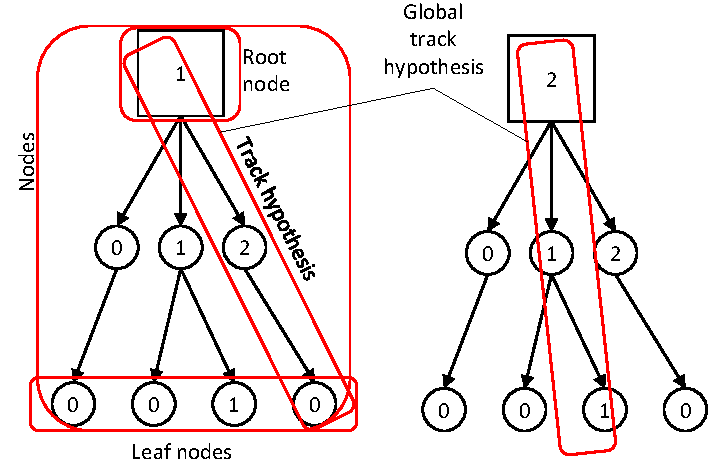
\includegraphics[clip, trim=0cm 2.5cm 0cm 2.5cm, width = .7\textwidth]{Track-tree}
\caption{Track hypothesis tree}
\label{fig:hyp-tree}
\end{figure}

\begin{equation}
\begin{split}
\M{A_1} &=\begin{bmatrix}
		0 & 1 & 1 & 0 & 0 & 0 & 0 & 0 & 0 \\
       	0 & 0 & 1 & 0 & 0 & 1 & 0 & 1 & 0 \\
       	0 & 0 & 0 & 1 & 0 & 0 & 1 & 1 & 1 \\
       	0 & 0 & 0 & 0 & 0 & 0 & 0 & 0 & 1 \\
     	\end{bmatrix}
\V{b_1} = 	\begin{bmatrix}
			1 \\ 1  \\ 1 \\ 1
			\end{bmatrix} \\
\M{A_2} &=\begin{bmatrix}
		1 & 1 & 1 & 1 & 0 & 0 & 0 & 0 & 0 \\
       	0 & 0 & 0 & 0 & 1 & 1 & 1 & 1 & 1 \\
     	\end{bmatrix} 
\V{b_2} = 	\begin{bmatrix}
			1 \\ 1
			\end{bmatrix} \\
\V{c} &=\begin{bmatrix}
		\lambda_1 & \lambda_2 & \lambda_3 & \lambda_4 & \lambda_5 & \lambda_6 & \lambda_7 & \lambda_8 & \lambda_9
		\end{bmatrix}^T \\
\end{split}
\label{eq:example_matrices}
\end{equation}

The explicit enumeration that becomes necessary when creating these $\M{A}$ matrices is exhaustive since the dimension of $\V{\tau}$, which is equal to the number of leaf nodes in the track forest, can be very large. Both $\M{A}_1$ and $\M{A}_2$ grows quadratically with the number of track hypotheses and real measurements or number of targets respectively.
% $N_1$ is proportional with the number of targets and history steps (N-scan). 

\subsection{Solvers}
There are a lot of off-the-shelf \gls{ilp} and \gls{milp} solvers on the marked, both free open source and commercial. Since the problem in this report is formulated on standard form, it can easily be executed on several solvers, and we can compare runtime and performance. The performance difference of some of these where tested in~\cite{Liland_2017}, where the difference where found marginal, probably because of the nature of the problem. %The read/write overhead, building problem vs. solving problem, etc. 


% \section{ILP Pruning}

\section{Dynamic window}

\section{N-Scan pruning}

\section{Track termination}